\documentclass{article}
\usepackage{ctex}
\usepackage{bm}
\usepackage[colorlinks, linkcolor=blue]{hyperref}
\usepackage{geometry}
\geometry{left=3cm, right=3cm, top=3cm, bottom=3cm}
\usepackage{amsmath}
\usepackage{amsthm}
\usepackage[T1]{fontenc}
\usepackage{xcolor}
\usepackage{lmodern}
\usepackage{listings}

\newtheorem{task}{问题}
\newtheorem*{proo}{证明}

\lstset{
	numbers=left, 
	numberstyle= \small, 
	keywordstyle= \color{ blue!70},
	commentstyle= \color{red!50!green!50!blue!50}, 
	frame=shadowbox, % 阴影效果
	showstringspaces = false,
	flexiblecolumns,                % 别问为什么,加上这个
	rulesepcolor= \color{ red!20!green!20!blue!20} ,
	escapeinside=``, % 英文分号中可写入中文
	breaklines=true,
	%xleftmargin=2em,xrightmargin=2em, aboveskip=1em,
	framexleftmargin=2.7em
}

\lstdefinestyle{Fortran}{
	language        =   [90]Fortran,
	basicstyle=\small\ttfamily
}

\title{作业五:数值积分}
\author{英才1701 赵鹏威 U201710152}

\begin{document}
	\maketitle
	\tableofcontents
%	\newpage
	\section{引言}
	科学计算中常常会碰到求积分的问题,但是能够求出不定积分的情况非常有限。如果要在不求出不定积分的情况下求出定积分,就可以使用数值积分方法. 本次作业使用两种数值积分方法:复合梯形积分和复合辛普森积分.
	
	\section{问题描述}
	\begin{task}
		使用复合梯形积分和复合辛普森积分计算
		\[
		\int_1^5\sin(x)\mathrm{d}x,
		\]
		要求步长为$h=0.1$,并估计误差.
	\end{task}
	这个积分可以求出真实值
	\[
	\int_1^5\sin(x)\mathrm{d}x=\cos(1)-\cos(5)\approx0.25664012.
	\]
	由于问题要求使用的步长为0.1,因此需要将$1$和$5$等分成$40$段,进行复合积分.
	
	\section{程序实现}
	\subsection{复合梯形积分}
	给定函数$f$,积分上下限$a$、$b$和整数$n$,复合梯形积分可以表示为
	\[
	T_n(f)=\frac{h}{2}\left(f(a)+2 \sum_{i=1}^{n-1} f\left(x_{i}\right)+f(b)\right),
	\]
	其中$h=(b-a)/n$,$x_i=a+ih$. 复合梯形积分的误差用下式计算
	\[
	E_n=\frac{4}{3}(T_{2n}-T_{n}).
	\]
	复合梯形积分的流程图如图\ref{fig:trapezoid}所示. 代码见 Listing.\ref{trapezoid.f90}
	\begin{figure}[h!tb]
		\centering
		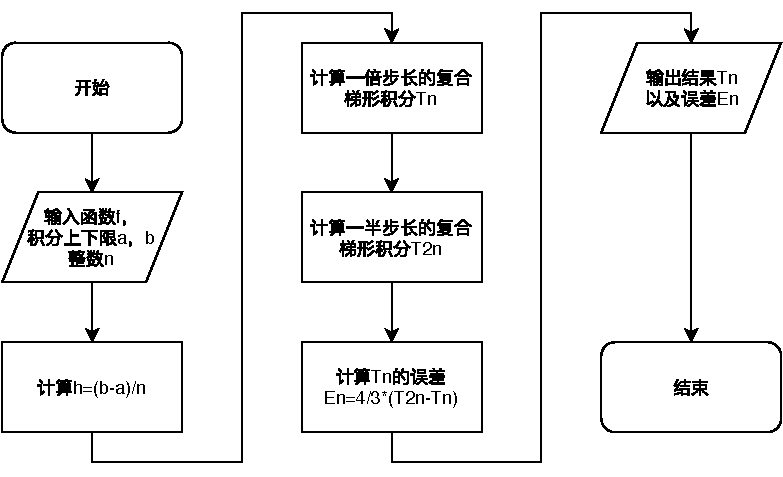
\includegraphics[width=1.0\textwidth]{./utils/trapezoid.pdf}
		\caption{ 复合梯形积分流程图\label{fig:trapezoid}}
	\end{figure}
	\lstinputlisting[
	style = Fortran,
	caption     =   {\bf trapezoid.f90},
	label       =   {trapezoid.f90}
	]{./utils/snips/trapezoid.f90}
	
	\subsection{复合辛普森积分}
	给定函数$f$,积分上下限$a$、$b$和偶数$n=2m$,复合梯形积分可以表示为
	\[
	S_{n}(f)=\frac{h}{3}\left(f(a)+4 \sum_{i=0}^{m-1} f\left(x_{2 i+1}\right)+2 \sum_{i=1}^{m-1} f\left(x_{2 i}\right)+f(b)\right).
	\]
	误差用下式计算
	\[
	E_n=\frac{16}{15}(S_{2n}-S_n).
	\]
	注意复合辛普森积分要求区间被分成偶数段,也就是$n$必须为偶数. 复合辛普森积分的流程图如图\ref{fig:simpson}所示. 代码见 Listing.\ref{simpson.f90}.
	\begin{figure}[h!tb]
		\centering
		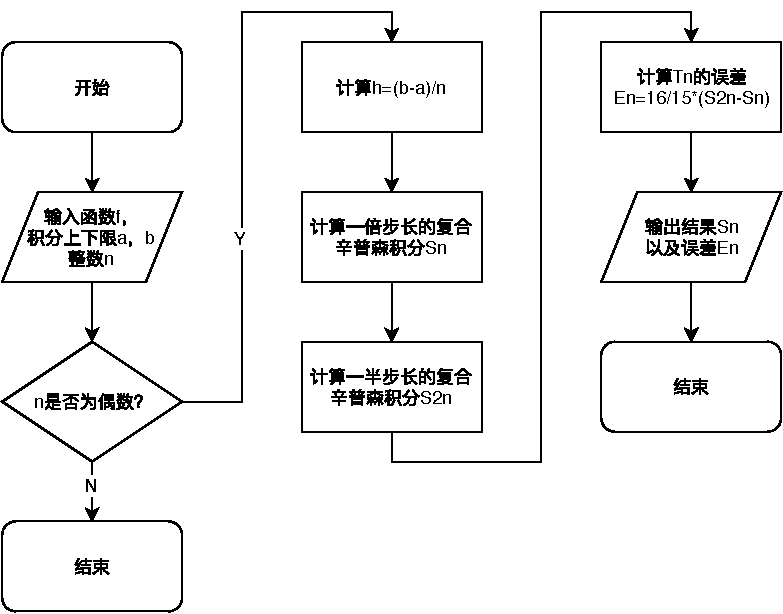
\includegraphics[width=1.0\textwidth]{./utils/simpson.pdf}
		\caption{ 复合辛普森积分流程图\label{fig:simpson}}
	\end{figure}
	\lstinputlisting[
	style = Fortran,
	caption     =   {\bf simpson.f90},
	label       =   {simpson.f90}
	]{./utils/snips/simpson.f90}
	
	\section{运行时结果}
	程序的运行时结果如图\ref{fig:rtr}所示. 第1列数字是积分结果,第2列数字是误差估计. 可以看到,与真值相比,复合梯形积分能够精确到小数点后第3位,而复合辛普森积分能够精确到小数点后第6位. 另外,可以发现,如果将两种方法计算出来的数值积分结果加上对于的误差估计,就能够很接近真值,可见误差估计非常准确.
	\begin{figure}[h!tb]
		\centering
		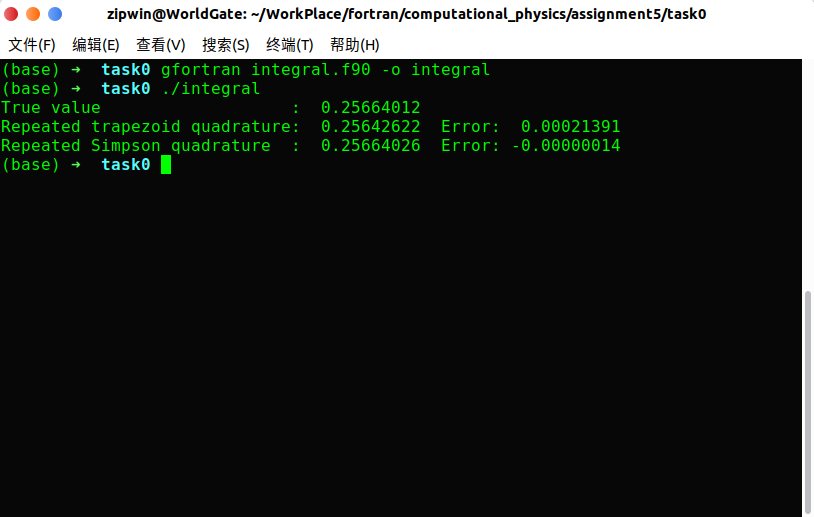
\includegraphics[width=1.0\textwidth]{./utils/rtr.png}
		\caption{ 运行时结果\label{fig:rtr}}
	\end{figure}
    	
	\section*{附录}
	代码可在\url{https://github.com/ZipWin/computational_physics/tree/master/assignments/assignment5}找到.
	\lstinputlisting[
	style = Fortran,
	caption     =   {\bf integral.f90},
	label       =   {integral.f90}
	]{./utils/integral.f90}
	
\end{document}
